\documentclass[journal,12pt,twocolumn]{IEEEtran}
\usepackage{tikz}
\usepackage{amsmath}
\usepackage{amssymb}
\pagestyle{empty}
\usepackage{setspace}
\singlespacing
\usepackage{caption}
\captionsetup{justification=centering}
\usepackage{amsthm}
\usepackage{amssymb,amsmath}


\begin{document}
\newcommand{\myvec}[1]{\ensuremath{\begin{pmatrix}#1\end{pmatrix}}}
\newcommand{\cmyvec}[1]{\ensuremath{\begin{pmatrix*}[c]#1\end{pmatrix*}}}
\providecommand{\norm}[1]{\lVert#1\rVert}
\newcommand{\mydet}[1]{\ensuremath{\begin{vmatrix}#1\end{vmatrix}}}
\newcommand{\proj}[2]{\textbf{proj}_{\vec{#1}}\vec{#2}}
\newcommand{\abs}[1]{\left\lvert#1\right\rvert}
\newcommand{\RNum}[1]{\uppercase\expandafter{\romannumeral #1\relax}}
\newcommand{\Rnum}[1]{\lowercase\expandafter{\romannumeral #1\relax}}
\let\StandardTheFigure\thefigure
\let\vec\mathbf

\title{
BASICS OF PROGRAMMING

ASSIGNMENT - 1
}
\author{ Sahin Hossain Chowdhury - SM21MTECH12002}
\maketitle
\newpage
\bigskip
\renewcommand{\thefigure}{\theenumi}
\bibliographystyle{IEEEtran}
\section*{ Chapter \RNum{2} Ex-\RNum{2} Q.3-\Rnum{2}}
\noindent

Showing That the following triads of points form right angled triangles or Not:
\begin{align}
\vec{A} = \myvec{2\\2}, \vec{B} =\myvec{6\\3},
\vec{C} =\myvec{4\\11}
\end{align}
\noindent
\section*{\textbf{Solution}}
\noindent
Pythagoras Theorem:=
\begin{equation}
Hypotenuse^2=Base^2+Height^2
\end{equation}
\begin{align}
\begin{split}
\norm{ \vec{A} - \vec{B}}^2 &= (\vec{A} - \vec{B})^T  
(\vec{A} - \vec{B} )\\
 \vec{A} - \vec{B} &= 
\myvec{2-6\\2-3} \\ &= 
\myvec{-4\\ -1} \nonumber  \\
\end{split}
\end{align}
\begin{equation}
\norm{ \vec{A} - \vec{B}} &= \sqrt{(-4)^2 + (-1)^2} =
4.1231
\end{equation}
\vspace{0.1cm}
\begin{align}
\begin{split}
\norm{ \vec{B} - \vec{C}}^2 &= (\vec{B} - \vec{C})^T 
(\vec{B} - \vec{C} )\\
 \vec{B} - \vec{C}
&= \myvec{6-4\\3-11} \\
&= \myvec{2\\ -8} \nonumber  \\
\end{split}
\end{align}
\begin{equation}
\norm{ \vec{B} - \vec{C}} &= \sqrt{(2)^2 + (-8)^2} =
8.2462
\end{equation}
\vspace{0.1cm}
\begin{align}
\begin{split}
\norm{ \vec{A} - \vec{C}}^2 &= (\vec{A} - \vec{C})^T  (\vec{A} - \vec{C} ) \\
 \vec{A} - \vec{C}
&= \myvec{2-4\\2-11} \\
&= \myvec{2\\ -9} \nonumber  \\
\end{split}
\end{align}
\begin{equation}
 \norm{ \vec{A} - \vec{C}} &= \sqrt{(2)^2 + (9)^2} 
=9.2195
\end{equation}

Maximum length is Hypotenuse
\begin{align}
Hypotenuse(AC)=9.2195\\
Base(AB)=4.1231 \\
Height(BC)=8.2462
\end{align}

Now To be An Right Angled Triangle:
\begin{equation}
    AC^2=AB^2+BC^2
\end{equation}
Here I Can See:
\begin{align}
    9.2195^2 = 4.1231^2+8.2462^2
\end{align}
So I Can Say That These Three Points(A,B,C)  forming Right Angled Triangle
\begin{figure}[!ht]
    \centering
    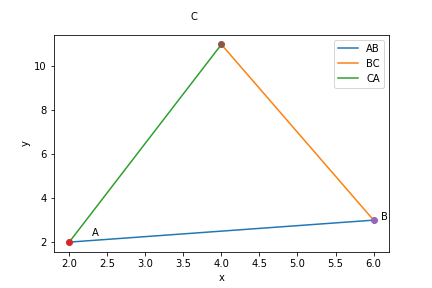
\includegraphics[width=\columnwidth]{Triangle.png}
    \caption{Triangle}
\end{figure}
\end{document}
